\chapter{Conclusiones}
\label{chap:conclusiones}
\section{Resultados}
\begin{figure}[h]
	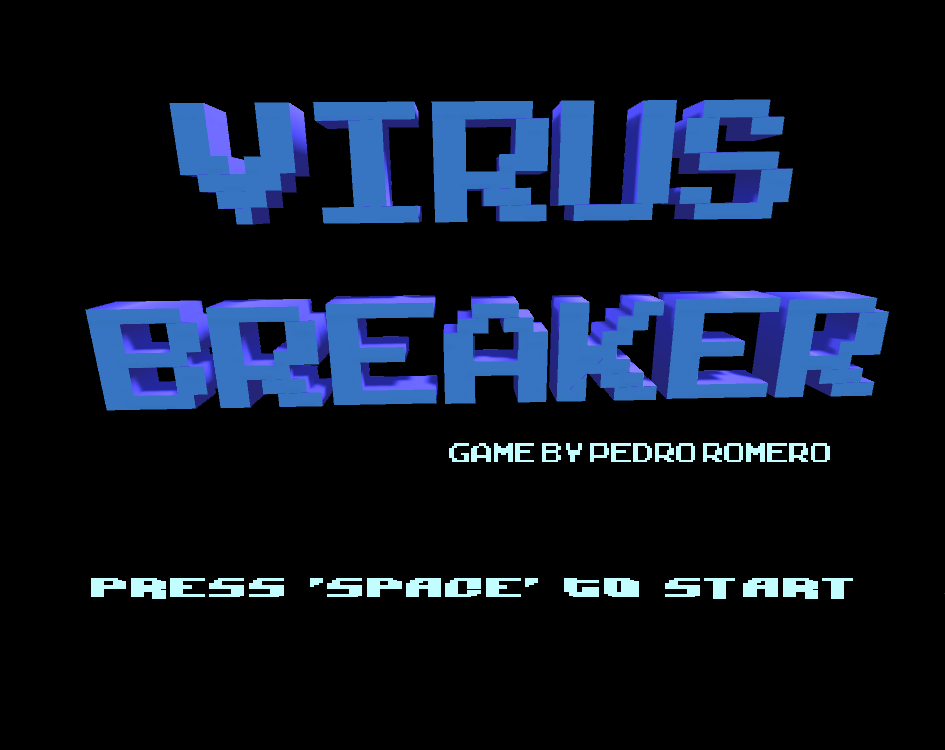
\includegraphics[width=0.8\textwidth]{images/futuro/resultado/captura-title}
	\centering
	\caption{Relación entre desafío y la ansiedad/aburrimiento.}
\end{figure}
El desarrollo del juego tuvo éxito en implementar las características básicas del juego. Algunas de estas características son: 
\begin{itemize}
\item El control de personaje principal fue desarrollado completamente, de forma que es preciso y fácil de controlar. Se pudo implementar unas pequeñas cinemáticas para su entrada y salida de la sala.
\item El movimiento de la pelota y su interacción con el resto de los elementos también fue implementado con éxito, incluyendo las modificaciones a las trayectorias de rebote naturales que mejoraban la experiencia de juego. 
\item La funcionalidad deseada para el sistema de carga de niveles pudo ser implementada a la perfección, con posibilidad de fácil ampliación en caso de necesidad.
\item Relacionado con los niveles, se pudieron implementar los cinco tipos de bloques descritos en el diseño.
\item El jefe final pudo ser implementado. 
\item Las pantallas de título y fin del juego pudieron ser implementadas y decoradas con textos animados. En adición a estas dos primeras pantallas, se creó una pantalla de victoria.
\end{itemize}

\begin{figure}[h]
	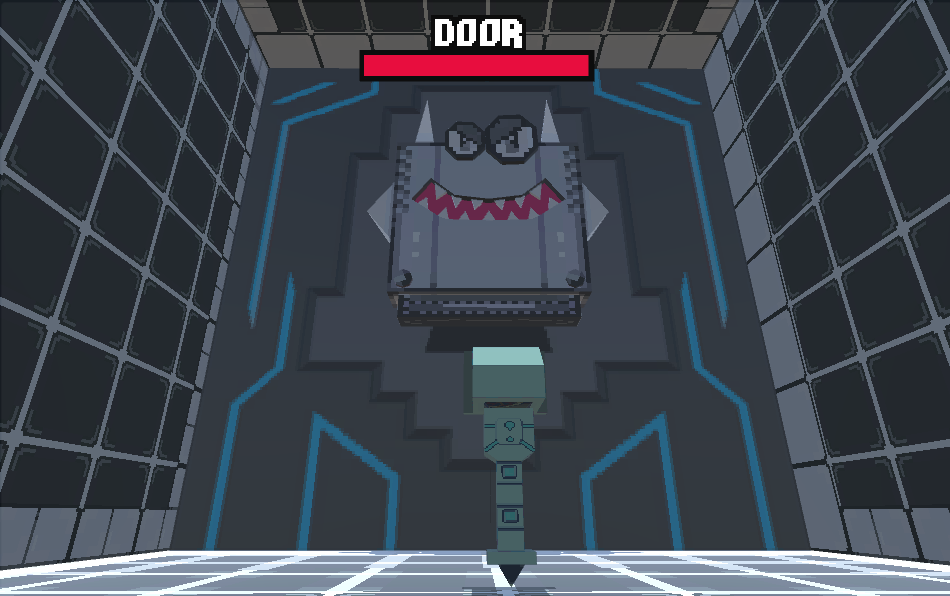
\includegraphics[width=0.8\textwidth]{images/futuro/resultado/captura-boss}
	\centering
	\caption{Relación entre desafío y la ansiedad/aburrimiento.}
\end{figure}

El estilo artístico del juego pudo ser implementado completamente. Todos los elementos del juego cuentan con su modelo y textura propios, gracias a la simpleza del estilo gráfico. También se añadieron pequeñas animaciones simples al personaje principal, a la puerta, al jefe y a los textos de los menús. Las partículas que se utilizan para enfatizar determinadas acciones, como el movimiento de la pelota o la destrucción de bloques, se implementaron utilizando texturas solidas de baja resolución, lo que conjuga con el resto del estilo. 

El juego se encuentra alojado tanto en GameJolt(https://gamejolt.com/games/virus\_breaker/316764) como en Itch.io(https://pedro-romero.itch.io/virus-breaker). En ambas páginas, el juego puede ser descargado gratuitamente para la plataforma Windows.

\begin{figure}[h]
	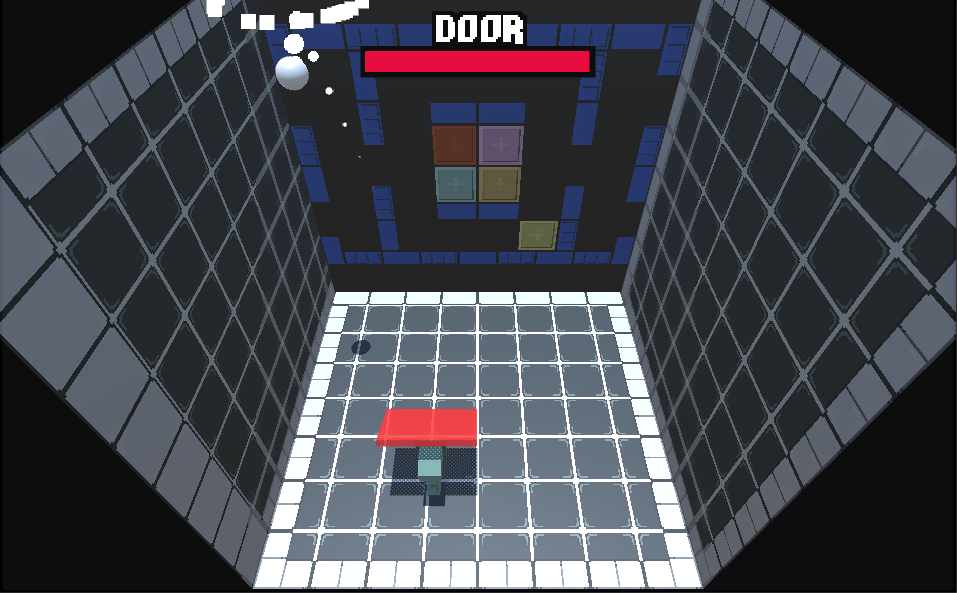
\includegraphics[width=0.8\textwidth]{images/futuro/resultado/captura-pacman}
	\centering
	\caption{Relación entre desafío y la ansiedad/aburrimiento.}
\end{figure}

\section{Mejoras Futuras}
Debido a las limitaciones de tiempo y alcance de este proyecto, el juego resultante está lejos de los estándares de calidad de la industria actual. En caso de querer retomar este proyecto por un estudio profesional, el juego debería ser modificado para añadir gráficos y sonidos de mejor calidad, aumentar su duración con más niveles y limpiar y optimizar su código.

A continuación, hablaremos de algunos de los elementos que podrían ser añadidos en versiones futuras del juego. Muchos de ellos son elementos que se idearon originalmente para formar parte de esta versión del proyecto, pero fueron descartados por falta de tiempo y recursos.

\subsection{Escenarios}
Lo primero que se añadiría al juego serían más niveles de juego. Al aumentar el número de niveles supondrá un incremento de la duración del juego, lo que resultará más atractivo para el jugador. Dado que los juegos de este género pueden superar el centenar de niveles (por ejemplo, LEGO Bricktopia\footnote{https://www.bigfishgames.com/games/1252/legobricktopia/} cuenta con 150 niveles) por lo que sería necesario implementar un número mayor de niveles para poder competir con ellos.

La cantidad de niveles que se pueden realizar no es infinita: solo alternando la configuración de los bloques que existe actualmente se llegará pronto a un punto en el que no se podrán crear más niveles sin caer en la repetición. La solución a este problema sería la implementación de más elementos de juego que dotaran de variedad a los niveles.

La creación de más tipos de bloques sería una de las primeras soluciones, ya que podrían integrarse con relativa facilidad al sistema actual de codificación de niveles. Entre los posibles bloques estarían los bloques explosivos (destruyen bloques cercanos al ser destruidos), bloques móviles que pudiesen programarse para crear formaciones móviles, o bloques con propiedades físicas distintas que alteraran el movimiento de la pelota (aumentando su velocidad o haciendo que rebote en ángulos extraños).

Otro posible elemento por implementar serían los niveles móviles. En estos la cámara se movería por una sala mucho más grande que la sala convencional. En estos niveles el objetivo del jugador sería más luchar contra el movimiento de la cámara para evitar quedar fuera del encuadre que el de abrir la puerta. Los principales problemas para implementar estos niveles serian:
\begin{enumerate}
\item Se debería modificar la forma en la que los niveles se guardan para dar soporte a la nueva información necesaria para estos niveles (principalmente, tamaño y velocidad de movimiento).  
\item Habría que cambiar la estructura de la sala base para dar soporte al tamaño variable.
\item Convendría implementar un sistema que gestionase la creación de bloques, el cual fuese creando los bloques según aparecen en el encuadre, y los elimine según se salgan de este, para optimizar el juego.
\end{enumerate}

\subsection{Enemigos}
Los enemigos son elementos del juego que dificultan activamente el progreso al jugador, proveyendo al jugador de desafíos que superar\cite{game_design_patters}. Los enemigos son comunes en este género de juegos (apareciendo incluso en títulos pioneros como Arkanoid (1986, Taito)) y permiten dar variedad e interactividad a los niveles del juego. El juego final incluye un único enemigo, el jefe final, aunque durante el desarrollo se barajó la opción de crear algunos enemigos, pero fue descartada para reducir el coste de su programación.

Los dos enemigos diseñados eran los siguientes:
\begin{itemize}
\item \textbf{El Trepador}: Se trataba de un enemigo con forma de gusano que reptaba a velocidad constante por la sala, pudiendo incluso trepar por el techo y paredes. Podía aturdir al personaje principal si este lo tocaba, por lo que el jugador debía esquivarlos mientras se movían por la sala.
\item \textbf{El Replicador}: Este enemigo se colocaría en la puerta e imitaría el aspecto de los bloques. Cada cierto tiempo, este enemigo crearía una copia de si mismo en un espacio libre cercano, por lo que el jugador debería darse prisa o acabarían "reparando" la pared. Estos enemigos podían ser destruidos si se les golpeaba con la pelota.
\end{itemize}

También sería necesario la adicción de jefes finales, para dar variedad a los desafíos finales. Durante el desarrollo se barajaron varios jefes finales distintos, pero fueron descartados en favor del jefe actual dado que solo se tenía tiempo para implementar uno. Estos diseños podrían recuperarse, se tendría que tener en cuenta el coste de implementar un jefe, cuyo comportamiento es bastante más complejo.

\subsection{Sistemas Complementarios}
Fuera del diseño de niveles, el juego necesita de ciertos sistemas complementarios que sirvan para prolongar su vida útil.

El primero de estos sistemas sería una tabla de puntuaciones. Las tablas de puntuaciones son unas listas que almacenan la puntuación que han alcanzado los jugadores al terminar el juego con el propósito de que puedan ser comparadas. La implementación de estas tablas, junto con la de un sistema de puntuación (que podría estar basado en factores como el tiempo de juego, cantidad de bloques destruidos o número de niveles superados) aumentaría enormemente la vida útil del juego ya que alentaría al jugador a que volviera a jugar con el propósito de superar su propia puntuación o la de otro jugador. Idealmente, la tabla de puntuaciones seria online, compartida entre todos los jugadores, pero eso supondría un coste adicional debido a la infraestructura necesaria.

El segundo sistema que podría implementarse para aumentar la vida útil del juego es un sistema de generación procedimental de niveles. Este sistema podría producir una cantidad de niveles infinita, lo que solucionaría el problema de la corta duración y reduciría el tiempo de desarrollo dedicado a la generación manual de niveles. Además, basándose en este sistema podrían implementarse otros sistemas complementarios, como un sistema de ``niveles diarios'' en la que todos los jugadores jugarían a un mismo grupo de niveles (sistema presente en juegos como \textit{The binding of Issac: Rebirth}(Nicalis, 2014) o \textit{Leap Day}(Nitrome, 2016).
